\chapter{Control}
The purpose of this chapter is to model the dynamical system 
of each UAV and describe the control strategies used to achieve the 
desired position and velocity, while ensuring stability and robustness.
The focus of our work is to localize the position of the 
avalanche victims, therefore the control task of the drones' flight 
is limited and interested mainly in controlling the altitude 
(mantaining a fixed height) and the horizontal positions
$x$ and $y$.

Each $j$-th UAV is modeled as a quadrotor vehicle, the most common 
multirotor aerial platform, characterized by four rotors attached 
to a rigid cross-shaped airframe. Each individual rotor generates 
both a forcet and a torque. The dynamics of each quadrotor are 
described using Euler-Newton laws of motion, with the motion 
expressed in terms of both the inertial frame \( F_g \) and the 
body frame \( F_b \).
As already mentioned, we have assumed the body frame $F_b$
to coincide with the receiver frame $F_r$, relative to the
the ARTVA equipment installed on the drone; therefore 
from now on we will denote the body frame with $F_r$.

% NON MI PIACE TROPPO QUESTO PARAGRAFETTO
% Control of this underactuated system brings more challenges
% wrt to wheeled robots \cite{model_quadrotor}.
% We begin by introducing the fundamental notations and conventions, 
% followed by the complete dynamical model of the UAV. A simplification 
% is then presented, which linearizes the system and allows the use of 
% Proportional-Derivative (PD) control strategies. Finally, the control 
% strategies used to regulate the quadrotor's position and velocity are 
% detailed, including both outer-loop position control and inner-loop 
% attitude control. Lastly, a geometric control strategy is introduced 
% for application to the complete quadrotor dynamics model.

% METTERE PARAGRAFETTO DOVE SI PARLA DELLE REFERENCES USATE
% PICCOLO SOTA

\section{Notations}
We introduce the notations and conventions used in this work 
to model the quadrotor dynamics and control. 
In particular, in Table~\ref{tab:notations} we introduce and 
summarize all the quantities and variables needed.
\begin{table}[h!]
    \centering
    \begin{tabular}{lll}
        \hline
        Symbol & Description & Units \\
        \hline
        \(g\) & gravitational acceleration constant, \( g \in \mathbb{R}_{\geq 0} \) & m/s\(^2\) \\
        \(m\) & mass of the quadrotor, \( m \in \mathbb{R}_{\geq 0} \) & kg \\
        \(x_r\) & position of the quadrotor along \(x\) (east) in \(F_g\) & m \\
        \(y_r\) & position of the quadrotor along \(y\) (north) in \(F_g\) & m \\
        \(z_r\) & position of the quadrotor along \(z\) (up) in \(F_g\) & m \\
        \(v_x\) & linear velocity along \(x\) in \(F_g\) & m/s \\
        \(v_y\) & linear velocity along \(y\) in \(F_g\) & m/s \\
        \(v_z\) & linear velocity along \(z\) in \(F_g\) & m/s \\
        \(p\) & roll rate in \(F_b\) & rad/s \\
        \(q\) & pitch rate in \(F_b\) & rad/s \\
        \(r\) & yaw rate in \(F_b\) & rad/s \\
        \(\phi\) & roll angle (rotation about \(x\)-axis) & rad \\
        \(\theta\) & pitch angle (rotation about \(y\)-axis) & rad \\
        \(\psi\) & yaw angle (rotation about \(z\)-axis) & rad \\
        \(T\) & total thrust generated by the propellers, \( T \in \mathbb{R}_{\geq 0} \) & N \\
        \hline
    \end{tabular}
    \caption{Quantities used to describe the quadrotor system.}
    \label{tab:notations}
\end{table}


%DA RIVEDERE O DA TOGLIERE
The laws of motion are described in both the global inertial frame \( F_g \) 
(particularly for translational dynamics) and the body frame 
\( F_r \) (in which the rotational dynamics are expressed more 
easily). The body right-hand frame \( F_r \) is fixed to the quadrotor 
(rotates with it), with its 
origin located at the center of mass.
Its axes are defined as in \cite{model_quadrotor}:
\noindent
\begin{itemize}
    \item The \( x \)-axis points forward along the quadrotor's direction 
    of motion.
    \item The \( y \)-axis points to the left wing.
    \item The \( z \)-axis points upwards, consistent with 
    the thrust direction.
\end{itemize}
% QUI È UN BORDELLO PERCHE LA Z CHE VA IN SU 
% È PRESA DALLA CITAZIONE MENTRE LA DIREZIONE DEGLI ASSI
% VIENE DA UN ALTRA ROBA CHE FACCIO?, dovrei fare una figura io
% METTERE FOTO QUADROTOR STILIZZATO
% OPPURE COPIARE IL TKZ DELLE FRAME E METTERE QUELLA CON SOLO
% INERZIALE E RECEIVER (BODY)
\begin{figure}[h]
    \centering
    %\includegraphics[width=0.8\textwidth]{quadrotor_diagram.png}
    \caption{Quadrotor diagram showing body and inertial frames.}
    \label{fig:quadrotor_diagram}
\end{figure}

\noindent
For the inertial frame, we adopt a convention that does not use 
the standard NED\footnote{NED stands for North-East-Down.} inertial 
reference frame, to ensure consistency throughout our work. 
Instead, the inertial frame \( F_g \) follows the ENU 
\footnote{ENU stands for East-North-Up.} 
convention (Figure \ref{fig:ENU}), where the 
\( z \)-axis points upward, away from the center of the Earth. The 
inertial frame \( F_g \) is fixed to the ground, with its origin at a 
reference point (the takeoff location), and its axes are defined as:
\begin{itemize}
    \item The \( x \)-axis points east.
    \item The \( y \)-axis points north.
    \item The \( z \)-axis points opposite the gravity vector.
\end{itemize}
The ENU local tangent plane is similar to NED, except for swapping 
"down" for "up" and \( x \) for \( y \), which is more intuitive for certain 
geographical and aerial applications.

\begin{figure}[h!]
    \centering
    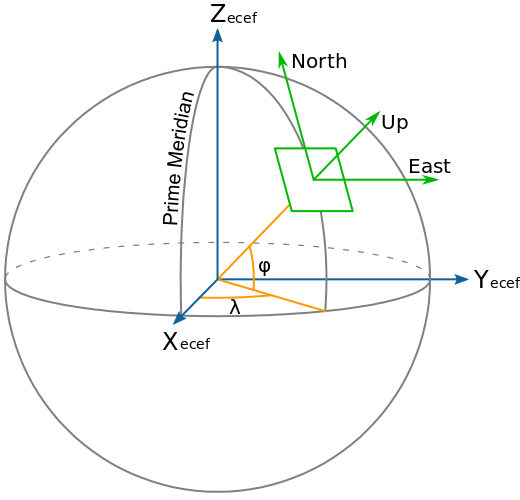
\includegraphics[width=0.5\textwidth]{images/ECEF_ENU_Longitude_Latitude_relationships.png}
    \caption[ENU and ECEF Reference Frames]{A diagram illustrating the ECEF (Earth-Centered, Earth-Fixed) 
    and ENU reference frames. 
    Adapted from a figure in \cite{ENU}.}
    \label{fig:ENU}
\end{figure}
%(IN REALTÀ È PRESA DA WIKI, VA BENE SI PUO FARE?)

\noindent
The orientation of the rigid body with respect to the inertial
frame is described by the rotation matrix 
\( \mathbf{R}^g_r(t) \in SO(3) \), which transforms vectors from the 
body frame \( F_r \) to the inertial frame \( F_g \).
The \( \mathbf{R}^g_r(t) \) rotation matrix is obtained by successive rotations around the 
inertial frame axes, these rotations define the roll, pitch and yaw angles \((\phi, \theta, \psi)\).
We specify the order of rotations as $x -y -z $:
\begin{itemize}
    \item yaw (\( \psi \)): rotation about the \(z\)-axis of the inertial frame \( F_g \).
    \item pitch (\( \theta \)): rotation about the \(y\)-axis of the inertial frame \( F_g \).
    \item roll (\( \phi \)): rotation about the \(x\)-axis of the inertial frame \( F_g \).
\end{itemize}
Since the successive rotations are relative to the fixed reference frame,
the full rotation matrix \( \mathbf{R}^g_r(t) \) is obtained as a product of the three individual rotation matrices:
\begin{align}
\mathbf{R}^g_r & = 
\mathbf{R}_z(\psi) \mathbf{R}_y(\theta) \mathbf{R}_x(\phi) \nonumber\\
& =
\begin{bmatrix}
\cos\psi & -\sin\psi & 0 \\
\sin\psi & \cos\psi & 0 \\
0 & 0 & 1
\end{bmatrix}
\begin{bmatrix}
\cos\theta & 0 & \sin\theta \\
0 & 1 & 0 \\
-\sin\theta & 0 & \cos\theta
\end{bmatrix}
\begin{bmatrix}
1 & 0 & 0 \\
0 & \cos\phi & -\sin\phi \\
0 & \sin\phi & \cos\phi
\end{bmatrix} \nonumber\\ 
& =
\resizebox{0.84\textwidth}{!}{$
\begin{bmatrix}
\cos\psi \cos\theta & \cos\psi \sin\theta \sin\phi - \sin\psi \cos\phi & \cos\psi \sin\theta \cos\phi + \sin\psi \sin\phi \\
\sin\psi \cos\theta & \sin\psi \sin\theta \sin\phi + \cos\psi \cos\phi & \sin\psi \sin\theta \cos\phi - \cos\psi \sin\phi \\
-\sin\theta & \cos\theta \sin\phi & \cos\theta \cos\phi
\end{bmatrix}
$}
\label{eq:attitude}
\end{align}
    
    
\noindent
\textbf{Note}
\\
Considering \( \mathbf{x} \in \mathbb{R}^3 \), we define a square matrix to 
be skew-symmetric \( \mathbf{S}(\mathbf{x}) \in \mathfrak{so}(3) \)
if and only if:
\begin{equation}
\mathbf{S}(\mathbf{x})\mkern-3mu^\top \mkern-4mu + \mathbf{S}(\mathbf{x}) = 0
\label{eq:skew_symmetric_condition}
\end{equation}
\noindent
Any rotation matrix \( \mathbf{R}(t) \in SO(3)\) satisfies the orthogonality condition:
\begin{equation}
\mathbf{R}(t) \, \mathbf{R}\mkern-3mu^\top\mkern-4mu(t) = \mathbf{I}
\label{eq:orthogonality_condition}
\end{equation}
\noindent
Computing the time derivative on both sides of \eqref{eq:orthogonality_condition} gives:
\begin{equation}
\dot{\mathbf{R}}(t) \, \mathbf{R}\mkern-3mu^\top\mkern-4mu(t) + \mathbf{R}(t) \, \dot{\mathbf{R}}\mkern-3mu^\top\mkern-4mu(t) = 0
\label{eq:time_derivative_orthogonality}
\end{equation}
\noindent
This is the skew-symmetry condition \eqref{eq:skew_symmetric_condition} 
for a matrix defined as:
\begin{equation}
\mathbf{S}(t) \stackrel{\Delta}{=} \dot{\mathbf{R}}(t) \, \mathbf{R}(t)\mkern-3mu^\top
\label{eq:def_skew_symmetric}
\end{equation}
\noindent
By postmultiplying $\mathbf{R}(t)$ on both sides of \ref{eq:def_skew_symmetric} we
obtain an expression for the variation in time of any rotation matrix:
\begin{equation}
\dot{\mathbf{R}}(t) = \mathbf{S}(t) \, \mathbf{R}(t)
\label{eq:skew_symmetric_rotation}
\end{equation}
\noindent
Since $\mathbf{R}(t)$ is the product of basic rotations with respect to the fixed frame and  
denoting with $ \boldsymbol{\omega}(t) = (\omega_x, \omega_y,  \omega_z)^\top \in \mathbb{R}^3$ the angular velocity of the body frame with respect to the fixed frame, 
we can repeat the same process to find an expression of $\mathbf{S}$ which depends on the time
derivative of the orientation angles, \cite{book-robotics}:
\begin{equation}
\mathbf{S}(\boldsymbol{\omega}) = 
\begin{bmatrix}
    0 & -\omega_z & \omega_y \\
    \omega_z & 0 & -\omega_x \\
    -\omega_y & \omega_x & 0
\end{bmatrix}
\label{eq:skew_symmetric_matrix}
\end{equation}
\noindent
Furthermore, the angular velocity of the rotating body frame with respect to the fixed frame is related with the angular velocity
expressed in the receiver frame as:
\begin{equation}
     \boldsymbol{\omega} = \mathbf{R}^g_r \, {}^r\mkern-3mu\boldsymbol{\omega}
    \label{eq:angular_velocity_inertial}
\end{equation}
\noindent
Then, we substitute Eq.\ref{eq:angular_velocity_inertial} in Eq.\ref{eq:def_skew_symmetric} to obtain the 
the skew-symmetric matrix of ${}^r \boldsymbol{\omega}$, in the body frame:
\begin{equation}
    \mathbf{S}(\boldsymbol{\omega}) =  \mathbf{S}(\mathbf{R}^g_r \, {}^r\mkern-3mu\boldsymbol{\omega}) 
    \label{eq:S_body}
\end{equation}
\noindent
Using the properties of skew-symmetric matrices:
\begin{equation}
    \mathbf{S}(\mathbf{R}^g_r \, {}^r\mkern-3mu\boldsymbol{\omega}) = \mathbf{R}^g_r \, \mathbf{S}({}^r\mkern-3mu\boldsymbol{\omega}) \, {\mathbf{R}^g_r}^\top 
    \label{eq:skew_symm_property}
\end{equation}
Substituting this result \eqref{eq:skew_symm_property} in Eq.\ref{eq:skew_symmetric_rotation}:
\begin{equation}
    \dot{\mathbf{R}^g_r} = \mathbf{R}^g_r \, \mathbf{S}({}^r\mkern-3mu\boldsymbol{\omega}) \, {\mathbf{R}^g_r}\mkern-3mu^\top  \, \mathbf{R}^g_r = \mathbf{R}^g_r \, \mathbf{S}({}^r\mkern-3mu\boldsymbol{\omega})
    \label{eq:skew_symmetric_body}
\end{equation}
We obtain the same expression of the inertial frame in the body frame.

\section{Complete Quadrotor Dynamics}
\subsection{Translational Dynamics}
Since the position of the UAV's center of gravity is represented by \( \mathbf{p}_r \in \mathbb{R}^3 \), 
expressed in the inertial frame \( F_g \), we denote its time derivative as \( \dot{\mathbf{p}}_r \) and 
the linear acceleration as \( \ddot{\mathbf{p}}_r \).
%VANNO MESSE LE COSE DELLE FORCE, COME SI TROVANO LE VELOCITÀ DEI MOTORI E 
%TUTTE QUESTE ALTRE COSE?
%%%%%%%%%%%%%% QUI C E COME CI SI ARRIVA
% Applying Newton's second law in the body frame, the translational dynamics are expressed as:
% \[
% m \frac{\mathrm{d}}{\mathrm{d}t}\mathbf{v}^b = \mathbf{f}^b,
% \]
% where:
% \begin{itemize}
%     \item \(\mathbf{v}^b = [v_x^b, v_y^b, v_z^b]^\top\): Linear velocity in the body frame.
%     \item \(\mathbf{f}^b\): Total force acting on the quadrotor, including thrust, drag, and gravity.
% \end{itemize}
% In the inertial frame, the translational dynamics of the quadrotor are given by:
% \[
% m \ddot{\mathbf{p}} = \mathbf{R}^\top \mathbf{f}^b - m g \mathbf{e}_z,
% \]
% where:
% \begin{itemize}
%     \item \(\ddot{\mathbf{p}}\): Acceleration of the quadrotor in the inertial frame.
%     \item \(\mathbf{e}_z = [0, 0, 1]^\top\): Unit vector in the \(z\)-direction of the inertial frame.
%     \item \(\mathbf{f}^b = [0, 0, f_{\text{thrust}}]^\top\): Force vector due to thrust in the body frame.
% \end{itemize}
% By transforming gravity into the body frame, we write:
% \[
% \mathbf{f}^b = \mathbf{R} \mathbf{f}^i,
% \]
% where \(\mathbf{f}^i\) includes gravitational and aerodynamic forces expressed in the inertial frame.


Then, by applying Newton-Euler first law, we obtain the 
translational dynamics of the quadrotor in the fixed inertial frame $F_g$ as in \cite{simplified_model}:
\begin{equation}
M \ddot{\mathbf{p}}_r = \sum \mathbf{F}_{\text{ext}} 
= T \, \mathbf{R}_r^g \, \mathbf{e}_z - M g \, \mathbf{e}_z - \mathbf{d}_f
\label{eq:translational_dyn}
\end{equation}
where \( \mathbf{F}_{\text{ext}} \) denotes all the external forces acting on the vehicle, which
includes the thrust force \( T \in \mathbb{R}_{\geq 0} \) generated by the propellers and therefore  
represents the control force, the input of the system which can be controlled.
It is aligned with the body \( z \)-axis by construction, as it is the sum of the single
forces generated by the aligned rotors. 
It also includes the gravitational force \( M g \), which instead is always directed towards the center of 
the Earth and therefore negative in our ENU fixed reference system. 
Finally, \( \mathbf{d}_f \) represents the disturbance forces, accounting for exogenous effects such as 
aerodynamic drag and wind disturbances \cite{control_quadrotor_main}.


\subsection{Rotational Dynamics}
%MANCA COME SI OTTENGONO LE TORQUES DAI MOTORI 
Newton-Euler's second law describes the variation in time of the angular momentum of a rigid body $\mathbf{L}$ 
in terms of the inertial reference frame, \cite{quadrotor_modeling_control_book}, \cite{book-robotics}:
\begin{equation}
    \frac{\mathrm{d} \mathbf{L}}{\mathrm{d}t} = \sum \boldsymbol{\tau}_{\text{ext}}
    \label{eq:NE-2}
\end{equation}
where \( \mathbf{L} \in \mathbb{R}^3 \) is the angular momentum of the rigid body,
expressed in the fixed inertial frame \( F_g \), and \( \boldsymbol{\tau}_{\text{ext}} \in \mathbb{R}^3 \) 
represents the total applied torque about the center of mass, which includes contributions 
from the control inputs, external disturbances, and aerodynamic effects.
\noindent \\
The angular momentum \( \mathbf{L} \) is related to the angular velocity as:
\begin{equation}
    \mathbf{L} = \mathbf{J} \, \boldsymbol{\omega}
    \label{eq:angular_momentum}
\end{equation}
where \( \mathbf{J} \in \mathbb{R}^{3 \times 3} \) is the inertia matrix of the rigid body, 
which is symmetric and positive definite (\( \mathbf{J} = \mathbf{J}^\top > 0 \)).
\noindent \\
However, it is more convenient to express the rotational dynamics 
in the body frame \( F_r \) of the rigid body, since the inertia matrix remains constant in this case. 
The opposite is not true, in fact the inertia matrix in the inertial frame is given by:
\begin{equation}
    \mathbf{J} =  \mathbf{R}^g_r \, {}^r\mkern-3mu\mathbf{J} \,  {\mathbf{R}^g_r}\mkern-2mu^\top 
    \label{eq:inertia_rot}
\end{equation}
Therefore, we substitute this property of the inertia matrix \eqref{eq:inertia_rot} and 
Eq.\ref{eq:angular_velocity_inertial} in Eq.\ref{eq:NE-2}, 
and use the result obtained earlier in \ref{eq:skew_symmetric_body}:
\begin{align}
    \frac{\mathrm{d} (\mathbf{J} \boldsymbol{\omega})}{\mathrm{d}t} &= 
    \dot{\mathbf{R}}^g_r \, {}^r\mkern-3mu\mathbf{J} \, {\mathbf{R}^g_r}\mkern-2mu^\top  {}^r\mkern-2mu\boldsymbol{\omega} +
    \mathbf{R}^g_r \, {}^r\mkern-3mu\mathbf{J} \, \dot{\mathbf{R}^g_r}\mkern-2mu^\top  {}^r\mkern-2mu\boldsymbol{\omega} \notag 
     + \mathbf{R}^g_r \, {}^r\mkern-3mu\mathbf{J} \, {\mathbf{R}^g_r}\mkern-2mu^\top  {}^r\mkern-2mu\dot{\boldsymbol{\omega}} \notag \\
    &= {}^r\mkern-3mu\mathbf{J} \, {}^r\dot{\boldsymbol{\omega}} + 
    {}^r\mkern-2mu\boldsymbol{\omega} \times ({}^r\mkern-3mu\mathbf{J} \, {}^r\mkern-2mu\dot{\boldsymbol{\omega}})
    \label{eq:derivazione_rotational_law}
\end{align}
\noindent\\
In the end, by comparing the right side of Eq.~\eqref{eq:derivazione_rotational_law}
with the right side of Eq.\ref{eq:NE-2}, we obtain as in \cite{control_quadrotor_main}
the complete rotational motion of the rigid body:
\begin{equation}
    {}^r\mkern-3mu\mathbf{J} \, {}^r\dot{\boldsymbol{\omega}} +
    {}^r\mkern-2mu\boldsymbol{\omega} \times ({}^r\mkern-3mu\mathbf{J} \, {}^r\mkern-2mu\dot{\boldsymbol{\omega}})
     = \sum \boldsymbol{\tau}_{\text{ext}}
    \label{eq:rot_dyn_final}
\end{equation}

\noindent\\
The inertia matrix \( {}^r\mkern-3mu\mathbf{J} \) depends on the geometry and mass distribution of the rigid body. 
For the quadrotor, assuming a rigid body structure with a dense spherical core of mass \( M \) and radius \( r \), 
along with four point masses \( m \) located at a distance \( l \) from the center, 
the inertia matrix takes the diagonal form:
\[
{}^r\mkern-3mu\mathbf{J} = 
\begin{bmatrix}
J_x & 0 & 0 \\
0 & J_y & 0 \\
0 & 0 & J_z
\end{bmatrix},
\]
where:
\[
J_x = J_y = \frac{2}{5} M r^2 + 2 l^2 m, \quad J_z = \frac{2}{5} M r^2 + 4 l^2 m.
\]
\noindent
Substituting Eq.~\eqref{eq:angular_momentum} into Eq.~\eqref{eq:rot_dyn_final}, we obtain the 
rotational dynamics law:
\begin{equation}
    {}^r\mkern-3mu\mathbf{J} \, {}^r\mkern-4mu\dot{\boldsymbol{\omega}} + {}^r\mkern-4mu\boldsymbol{\omega} \times 
    ({}^r\mkern-3mu\mathbf{J} \, {}^r\mkern-4mu\boldsymbol{\omega}) = \boldsymbol{\tau}_{\text{u}} + \mathbf{d}_{\tau}
    \label{eq:rotational_dynamics}
\end{equation}
where $\boldsymbol{\tau}_{\text{u}} \in \mathbb{R}^3$ is the controlled input
torque vector dependent on the single torque generated
by each rotor and with $\mathbf{d}_{\tau}$ we denote 
all the external disturbances.

\noindent\\
In addition, we need to relate the angular velocity \( {}^r\mkern-4mu\boldsymbol{\omega} \) in the body frame 
to the time derivatives of the roll, pitch and yaw angles (\( \phi, \theta, \psi \)) 
in the inertial frame. We assume that the variation of the angles  $\dot{\phi}, \dot{\theta}, \dot{\psi}$
is small and therefore $\dot{\mathbf{R}}_x(\phi) = \dot{\mathbf{R}}_x(\theta) =  \dot{\mathbf{R}}_x(\psi) = \mathbf{I}$:
\begin{equation}
    {}^r\boldsymbol{\omega} = 
    \begin{pmatrix}
        p \\ q \\ r
    \end{pmatrix}
    =
    \begin{pmatrix}
        1 & 0 & -\sin\theta \\
        0 & \cos\phi & \sin\phi\cos\theta \\
        0 & -\sin\phi & \cos\phi\cos\theta
    \end{pmatrix}
    \begin{pmatrix}
        \dot{\phi} \\ \dot{\theta} \\ \dot{\psi}
    \end{pmatrix}
    \label{eq:angular_rates_to_rpy}
\end{equation}

\noindent\\
Finally, also the rotation matrix \( \mathbf{R}_r^g (t) \) 
evolves in time as the rigid body rotates in space, following the result obtained earlier
in Eq.\ref{eq:skew_symmetric_body}:
\begin{equation}
    \dot{\mathbf{R}}_r^g = \mathbf{R}_r^g \, \mathbf{S}({}^r\boldsymbol{\omega})
    \label{eq:rotation_matrix_dynamics_final}
\end{equation}
where \( \mathbf{S}({}^r\mkern-4mu\boldsymbol{\omega}) \) is a skew-symmetric matrix
in the form of \eqref{eq:skew_symmetric_matrix}, but relative to the body frame components:
\begin{equation}
    \mathbf{S}({}^r\mkern-3mu\mathbf\boldsymbol{\omega}) = 
    \begin{bmatrix}
        0 & -r & q \\
        r & 0 & -p \\
        -q & p & 0
    \end{bmatrix}
\label{eq:skew_symmetric_matrix_body}
\end{equation}

\subsection{Final Complete Quadrotor Dynamics}
Combining the translational and rotational dynamics, the complete UAV dynamics is given by the system of equations
\ref{eq:translational_dyn}, \ref{eq:rotation_matrix_dynamics_final} and \ref{eq:rotational_dynamics}:
\begin{equation}
\begin{cases}
    M \ddot{\mathbf{p}}_r = T \, \mathbf{R}_r^g \, \mathbf{e}_z - M g \, \mathbf{e}_z - \mathbf{d}_f \\[6pt]
    \dot{\mathbf{R}}_r^g = \mathbf{R}_r^g \, \mathbf{S}({}^r\mkern-4mu\boldsymbol{\omega}) \\[6pt]
    {}^r\mkern-4mu\mathbf{J} \, {}^r\mkern-4mu\dot{\boldsymbol{\omega}} = 
    - {}^r\mkern-4mu\boldsymbol{\omega} \times 
    ({}^r\mkern-4mu\mathbf{J} \, {}^r\mkern-4mu\boldsymbol{\omega}) + \boldsymbol{\tau}_{\text{u}} + \mathbf{d}_{\tau}   
\end{cases}
\label{eq:final_model}
\end{equation}
More explicitly we can expand these equations and thanks to inverting Eq.\ref{eq:angular_rates_to_rpy}
and how we defined rotation matrix $\mathbf{R}_r^g$ in Eq.\ref{eq:attitude}, we obtain
a system with twelve states and four control inputs:
{\large
\begin{equation}
    \begin{cases}
        \dot{x}_r = v_x \\[6pt]
        \dot{y}_r = v_y \\[6pt]
        \dot{z}_r = v_z \\[6pt]
        \dot{v_x} = -d_{f,x} + (\cos(\psi) \sin(\theta) \cos(\phi) + \sin(\psi) \sin(\phi)) \frac{T}{M} \\[6pt]
        \dot{v_y} = -d_{f,y} + (\sin(\psi) \sin(\theta) \cos(\phi) - \cos(\psi) \sin(\phi)) \frac{T}{M} \\[6pt]
        \dot{v_z} = -d_{f,z} - g + \cos(\theta) \cos(\phi) \frac{T}{M} \\[6pt]
        \dot{\phi} = p + \sin(\phi) \tan(\theta) q + \cos(\phi) \tan(\theta) r \\[6pt]
        \dot{\theta} = \cos(\phi) q - \sin(\phi) r \\[6pt]
        \dot{\psi} = \sin(\phi) \sec(\theta) q + \cos(\phi) \sec(\theta) r \\[6pt]
        \dot{p} = \tau_{\phi} + \frac{I_y - I_z}{I_x} qr + \frac{\tau_\phi}{I_x} \\[8pt]
        \dot{q} = \tau_{\theta} + \frac{I_z - I_x}{I_y} pr + \frac{\tau_\theta}{I_y} \\[8pt]
        \dot{r} = \tau_{\psi} + \frac{I_x - I_y}{I_z} pq + \frac{\tau_\psi}{I_z}
    \end{cases}
    \label{eq:final_model_more}
\end{equation}}
\noindent
where $\tau_{\phi}, \tau_{\theta}, \tau_{\psi}$  are the components of input
torque vector $\boldsymbol{\tau}_{\text{u}} = (\tau_{\phi}, \tau_{\theta}, \tau_{\psi})^\top $.
\noindent
\\
In a compact state-space form:
\begin{equation}
    \dot{\boldsymbol{\xi}} = f(\boldsymbol{\xi}) + g(\boldsymbol{\xi}) \boldsymbol{u}
\end{equation}
where:
\[
\boldsymbol{\xi} = [x_r, y_r, z_r, v_x, v_y, v_z, \phi, \theta, \psi, p, q, r]^\top
\]
\[
\boldsymbol{u} = [T, \tau_\phi, \tau_\theta, \tau_\psi]^\top
\]
The non-linear dynamics of the state is desbribe by \( f(\boldsymbol{\xi}) \), 
while \( g(\boldsymbol{\xi}) \) represents the control input relationships
with the system.


\section{Simplified Dynamics}
To facilitate control design, we consider a simplified model of the quadrotor dynamics,
as proposed in \cite{simplified_model}. 
This model assumes nominal conditions with no external 
disturbances and employs a small angle approximation 
for the roll (\( \phi \)) and pitch (\( \theta \)) angles. 
Additionally, we assume symmetric mass distribution 
and negligible aerodynamic and gyroscopic effects.
\noindent
Under these assumptions:
\begin{itemize}
    \item Small angular velocities and small angles allow \( (\dot{\phi}, \dot{\theta}, \dot{\psi}) \approx (p, q, r) \),
     simplifying the rotational dynamics.
    \item The Coriolis or gyroscopic term  \( {}^r\boldsymbol{\omega} \times (\mathbf{J} \, {}^r\boldsymbol{\omega}) \) 
    in the rotational dynamics is negligible for stabilization tasks, where angular velocities remain small.
\end{itemize}
The simplified dynamics are:
\begin{equation}
\begin{cases}
    M \ddot{\mathbf{p}}_r = T \, \mathbf{R}_r^g \, \mathbf{e}_z - M g \, \mathbf{e}_z \\[6pt]
    \mathbf{J} \, {}^r\mkern-4mu\dot{\boldsymbol{\omega}} = \boldsymbol{\tau}_{\text{u}}
\end{cases}
\label{eq:simplified_rotational_dynamics}
\end{equation}
Explicitly expanded as:
\begin{subequations}
\begin{align}
    \ddot{x}_r &= (\cos\psi \sin\theta \cos\phi + \sin\psi \sin\phi) \frac{T}{M} \label{eq:position_control_x}\\[6pt] 
    \ddot{y}_r &= (\sin\psi \sin\theta \cos\phi - \cos\psi \sin\phi) \frac{T}{M} \label{eq:position_control_y}\\[6pt] 
    \ddot{z}_r &= \cos\theta \cos\phi \frac{T}{M} - g  \label{eq:position_control_z}\\[6pt] 
    \dot{\phi} &= \frac{\tau_{\phi}}{I_x} \\[8pt]
    \dot{\theta} &= \frac{\tau_{\theta}}{I_y} \\[8pt]
    \dot{\psi} &= \frac{\tau_{\psi}}{I_z}
\end{align}
\label{eq:simplified_model}
\end{subequations}
This simplified model reduces the complexity of the quadrotor dynamics,
making it adapt to be controlled by simple control strategies such as 
PID\footnote{PID stands for Proportional-Integral-Derivative} control.

%FIND CITATIONS FOR THE CONTROL PART 
%AND PLOT THE BLOCK DIAGRAM
\section{PD Control}
In this section, we implement a PID controller 
based on the simplified model from Section~\ref{eq:simplified_model}. 
The primal objective is to regulate the altitude $z$ and the 
horizontal positions \( x \) and \( y \) of the quadrotor along a 
specified trajectory $\mathbf{x}_d(t) \in \mathbb{R}^3$.
In order to do so we define position error $\mathbf{e}(t) \in \mathbb{R}^3$
between the actual position $p_r(t)$ f the $j$-th UAV and the desired trajectory as:
\[
    \mathbf{e}(t) = \mathbf{x}_d(t) - \mathbf{p}_r(t) = 
    \begin{bmatrix}
        e_x(t) \\
        e_y(t) \\
        e_z(t)
    \end{bmatrix} =
    \begin{bmatrix}
        x_d(t) - p_{r_x}(t) \\
        y_d(t) - p_{r_y}(t) \\
        z_d(t) - p_{r_z}(t)
    \end{bmatrix}
\]

\subsection{Altitude Hold}
Focusing firstly on the altitude $z$,
we drive the error esponentially to zero by controlling the acceleration
vector of the quadrotors $\ddot{z}_r$ as in \cite{simplified_model} to satisfy:
\[
 K_{p_z} ( z_r - z_d )  + K_{d_z} (\dot{z}_r - \dot{z}_d ) + \ddot{z}_r - \ddot{z}_d = 0
\]
\noindent
Therefore, the virtual input of our control system is:
\begin{equation}
    \ddot{z}_r  =  K_{p_z} e_z + K_{d_z} \dot{e}_z + \ddot{z}_d
    \label{eq:virtual_input}
\end{equation}
where \( K_{p_z} \) and \( K_{d_z} \) are the  proportional and derivative gains, respectively.

\noindent
From the simplified dynamics \eqref{eq:position_control_z}, 
the control thrust \( T \) required to maintain the altitude is given by:
\begin{equation}
    T = \frac{M}{\cos\theta \cos\phi} \, (g + \ddot{z}_r)
    \label{eq:true_input}
\end{equation}
\noindent
Substituting \( \ddot{z}_r \) from Eq.\ref{eq:virtual_input} in Eq.\ref{eq:true_input},
we obtain:
\[
T = \frac{M}{\cos\theta \cos\phi} \, \left( g + K_{p_z} e_z + K_{d_z} \dot{e}_z + \ddot{z}_d \right)
\]
%Since we do not need any vertical acceleration we specify $\ddot{z}_d = 0$, questo dillo nell implementazione.
%nell implementazione dire che la traiettoria scelat è una TRAIETTORIA ESPONENZIALE 

\subsection{Position Control}
The control strategy we have adopted is hierarchical since we have given priority to the 
altitude control to determine the desired input thrust; only after we determine this quantity
we define in cascade the control torques $\tau\theta, \tau\phi, \tau\psi$.
As before we want the position error to esponentially converge to zero,
therefore we desire:
\begin{equation}
    \begin{cases}
        K_{p_x} ( x_r - x_d )  + K_{d_x} (\dot{x}_r -\dot{x}_d) + \ddot{x}_r -\ddot{x}_d  = 0 \\[6pt]
        K_{p_y} (y_r - y_d )  + K_{d_y} ( \dot{y}_r - \dot{y}_d) +  \ddot{y}_r - \ddot{y}_d = 0
    \end{cases}
\end{equation}
where $K_{p_x}$ and $K_{p_y}$ are proportional gains, and $K_{d_x}$ and $K_{d_y}$ are derivative gains.
\noindent \\
From the simplified translational dynamics, Equations \ref{eq:position_control_x}
and \ref{eq:position_control_y}, we find the desired pitch \( \theta_d \) 
and roll \( \phi_d \) angles that ensure the system converges to the desired trajectory.
We substitute the desired angles and obtain:
\begin{subequations}
    \begin{align}
    \frac{M}{T} \ddot{x}_r &= \cos\psi \sin\theta \cos\phi + \sin\psi \sin\phi \label{eq:T_x} \\[6pt]
    \frac{M}{T} \ddot{y}_r &= \sin\psi \sin\theta \cos\phi - \cos\psi \sin\phi \label{eq:T_y}
    \end{align}
\end{subequations}

\noindent
After performing algebraic and trigonometric manipulations, we derive expressions for the desired roll and pitch angles:
\begin{equation}
    \phi_d =  \arcsin\left(  (T_y \cos\psi - T_x \sin\psi) \right)
\end{equation}
\begin{equation}
    \theta_d = - \arcsin\left(\frac{T_x \cos\psi + T_y \sin\psi}{ \cos\phi_d } \right)
\end{equation}
where $T_x = \frac{M}{T} \ddot{x}_r$ and $T_y = \frac{M}{T} \ddot{y}_r$ are the
desired components of the thrust vector in $x$ and $y$ and are found
using Equations \ref{eq:T_x} and \ref{eq:T_y} respectively.

\noindent\\
For the desired yaw angle, we use the relationship between the velocity 
components, so that the quadrotor mantains the correct heading direction.
Specifically, the yaw angle is determined as:
\begin{equation}
    \psi_d = \arctan2(\dot{y}_d, \dot{x}_d),
\end{equation}

\noindent
Using the desired angles $\phi_d$, $\theta_d, \psi_d$, the control torques are defined as:
\begin{equation}
    \tau_\phi = I_x \left(  K_{p_\phi} e_\phi + K_{d_\phi} \dot{e}_\phi \right)
\end{equation}
\begin{equation}
    \tau_\theta = I_y \left(K_{p_\theta} e_\theta + K_{d_\theta} \dot{e}_\theta \right)
\end{equation}
\begin{equation}
    \tau_\psi = I_z \left(K_{p_\psi} e_\psi + K_{d_\psi} \dot{e}_\psi \right)
\end{equation}
Where $K_{p_\phi}$, $K_{d_\phi}$, $K_{p_\theta}$, $K_{d_\theta}$, $K_{p_\psi}$, and $K_{d_\psi}$ 
represent the proportional and derivative gains for roll, pitch, and yaw, respectively. 
While the input force was defined earlier in Eq.\ref{eq:true_input}.

\subsection{Results}
The results of PID control with the simplified model \eqref{eq:simplified_model}
applied to trajectory tracking during the first positioning 
(exploration) phase of the algorithm, are shown in  Figures
\ref{fig:pid_sim}, \ref{fig:pd_traj_comparison}, \ref{fig:pid_x},
\ref{fig:pid_y}, \ref{fig:pid_z}.
\begin{figure}[h!]
    \centering
     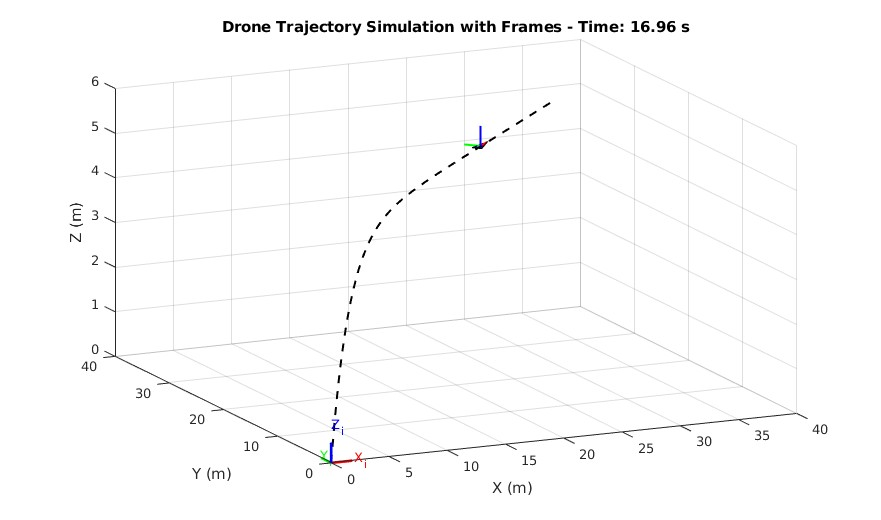
\includegraphics[width=1\textwidth]{images/pd_sim.jpg}
    \caption[Caption for Figure 1]{Simulation time frame}
    \label{fig:pid_sim}
\end{figure}
\begin{figure}[h!]
    \centering
     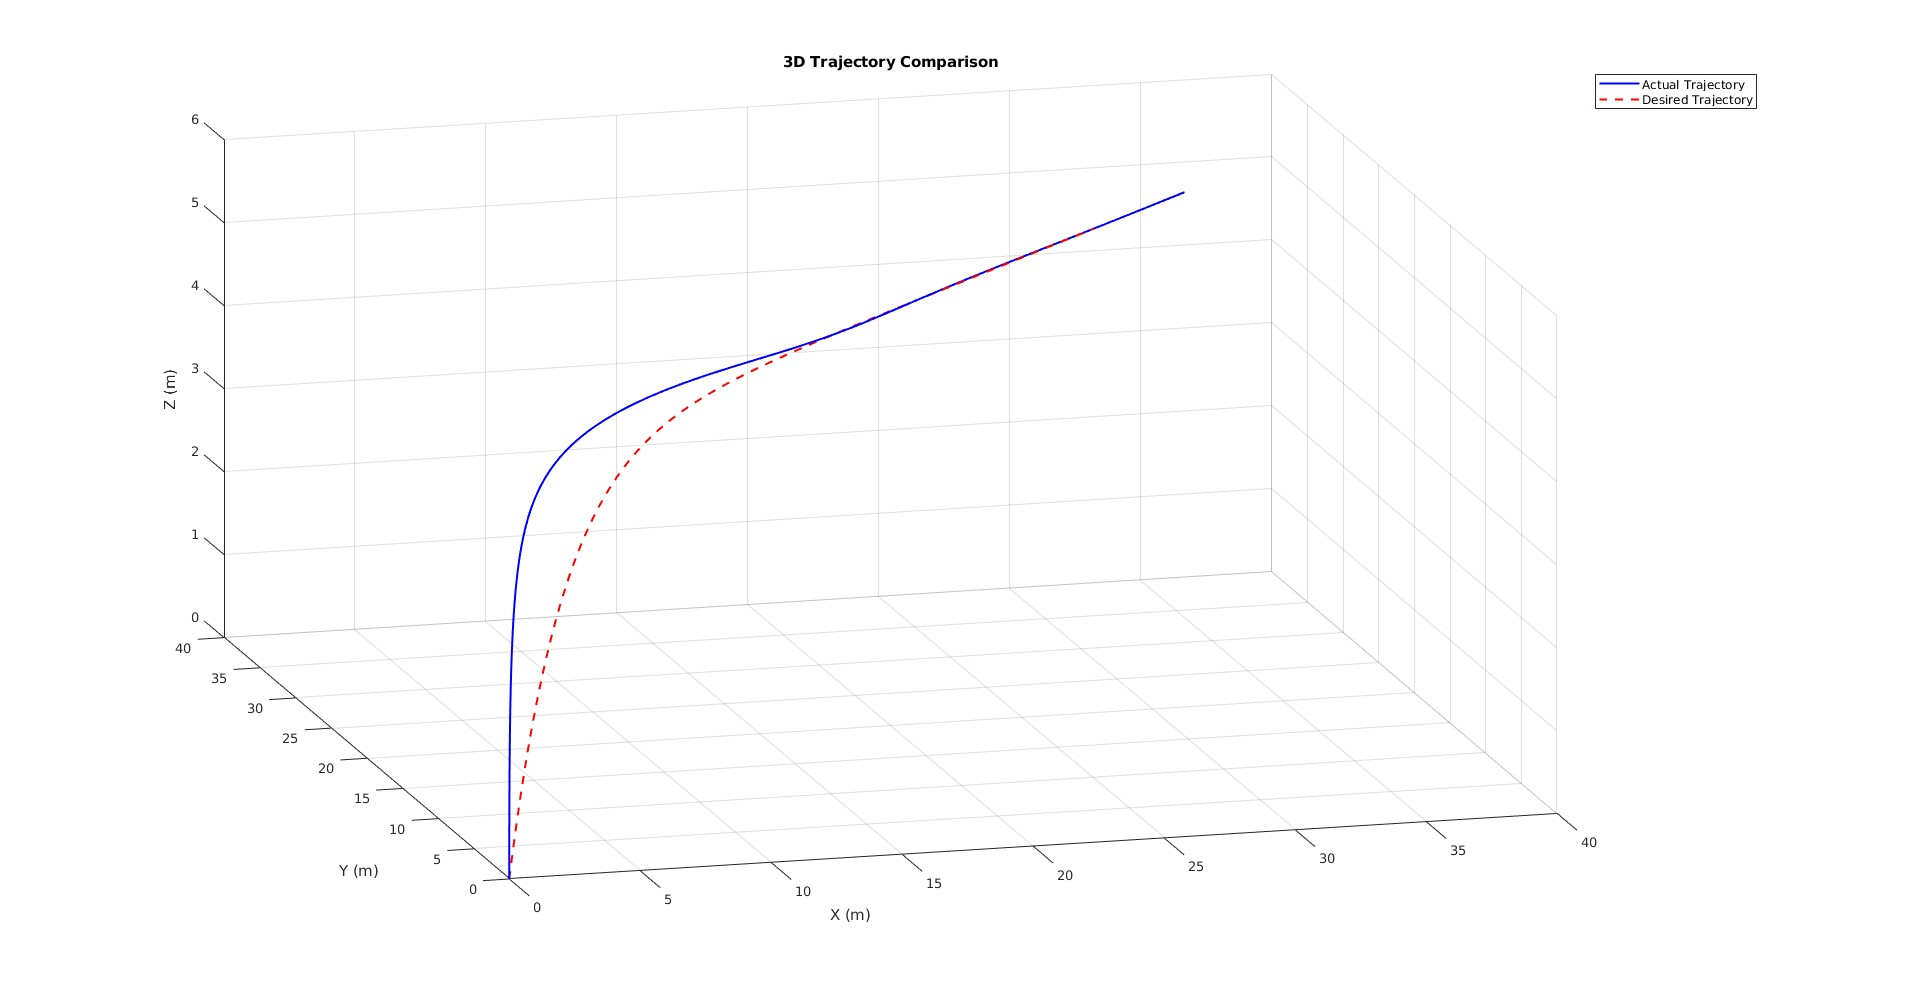
\includegraphics[width=1\textwidth]{images/pd_traj_comparison.jpg}
    \caption[Caption for Figure 2]{Actual and desired tarjectory in 3D space}
    \label{fig:pd_traj_comparison}
\end{figure}
\begin{figure}[h!]
    \centering
     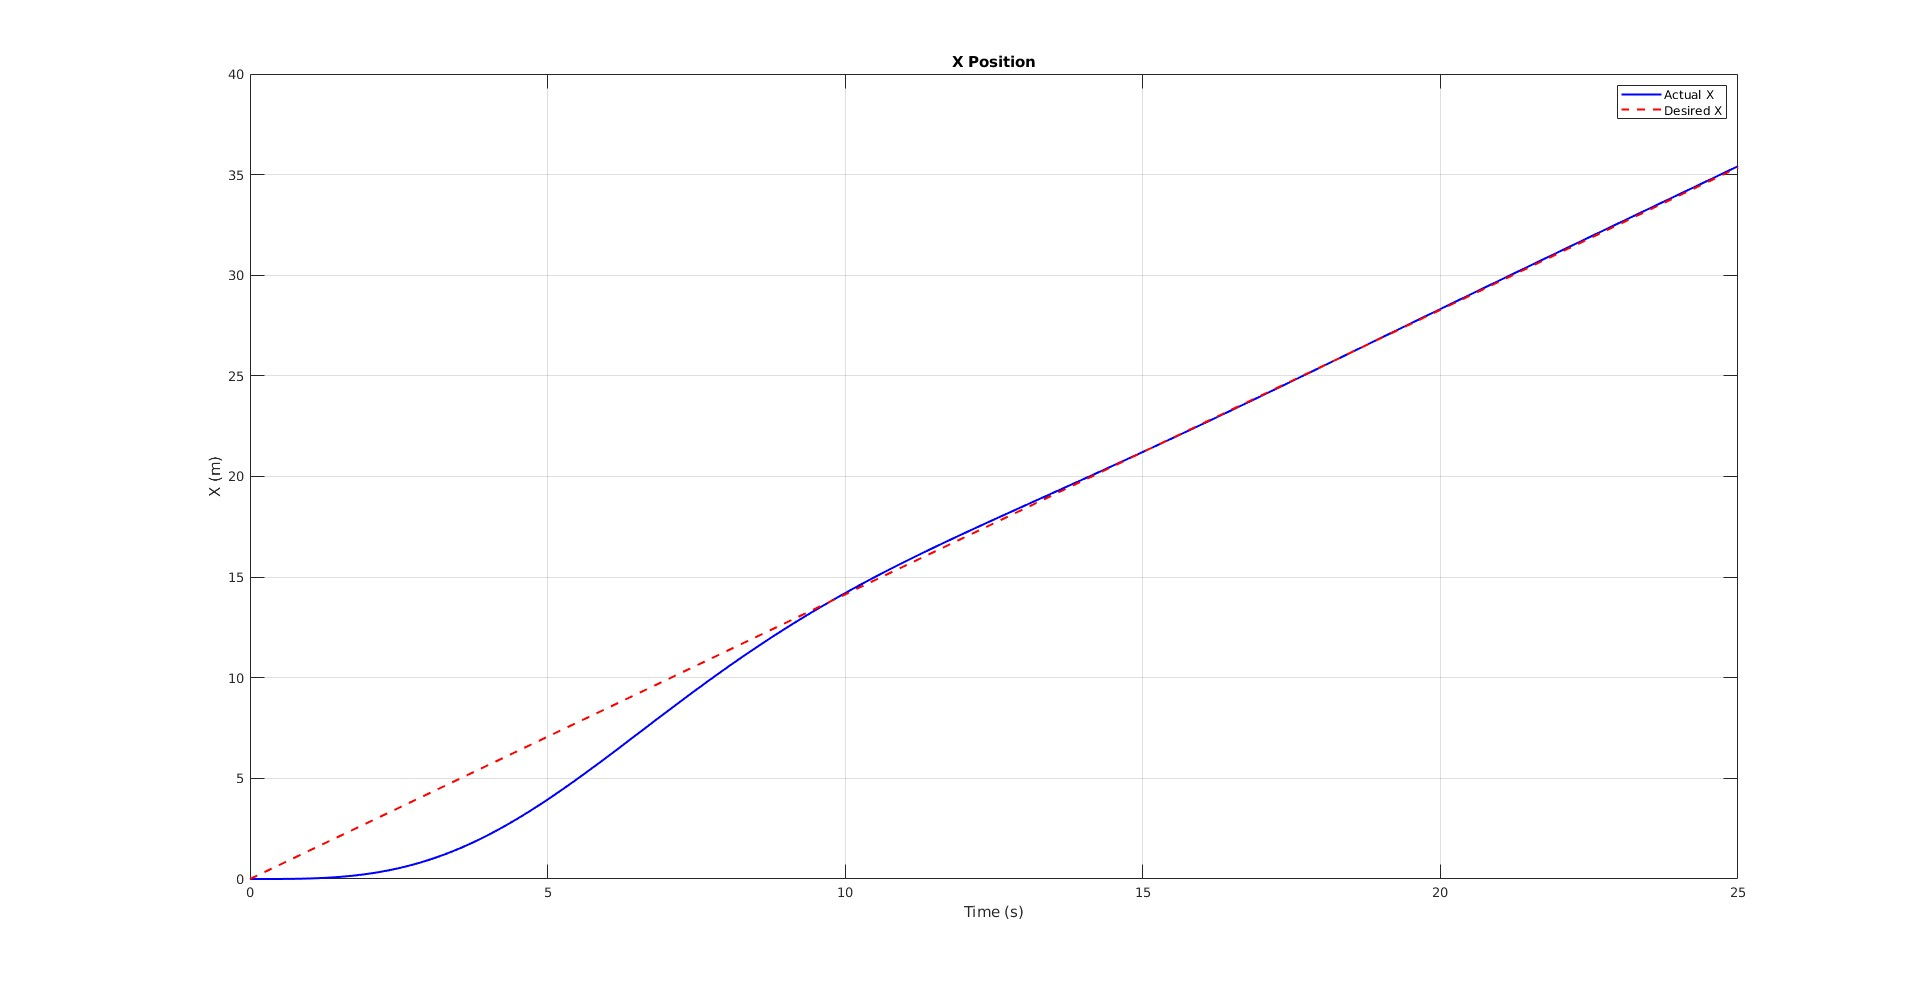
\includegraphics[width=1\textwidth]{images/pd_x.jpg}
    \caption[Caption for Figure 3]{Actual and desired $x$ position}
    \label{fig:pid_x}
\end{figure}
\begin{figure}[h!]
    \centering
     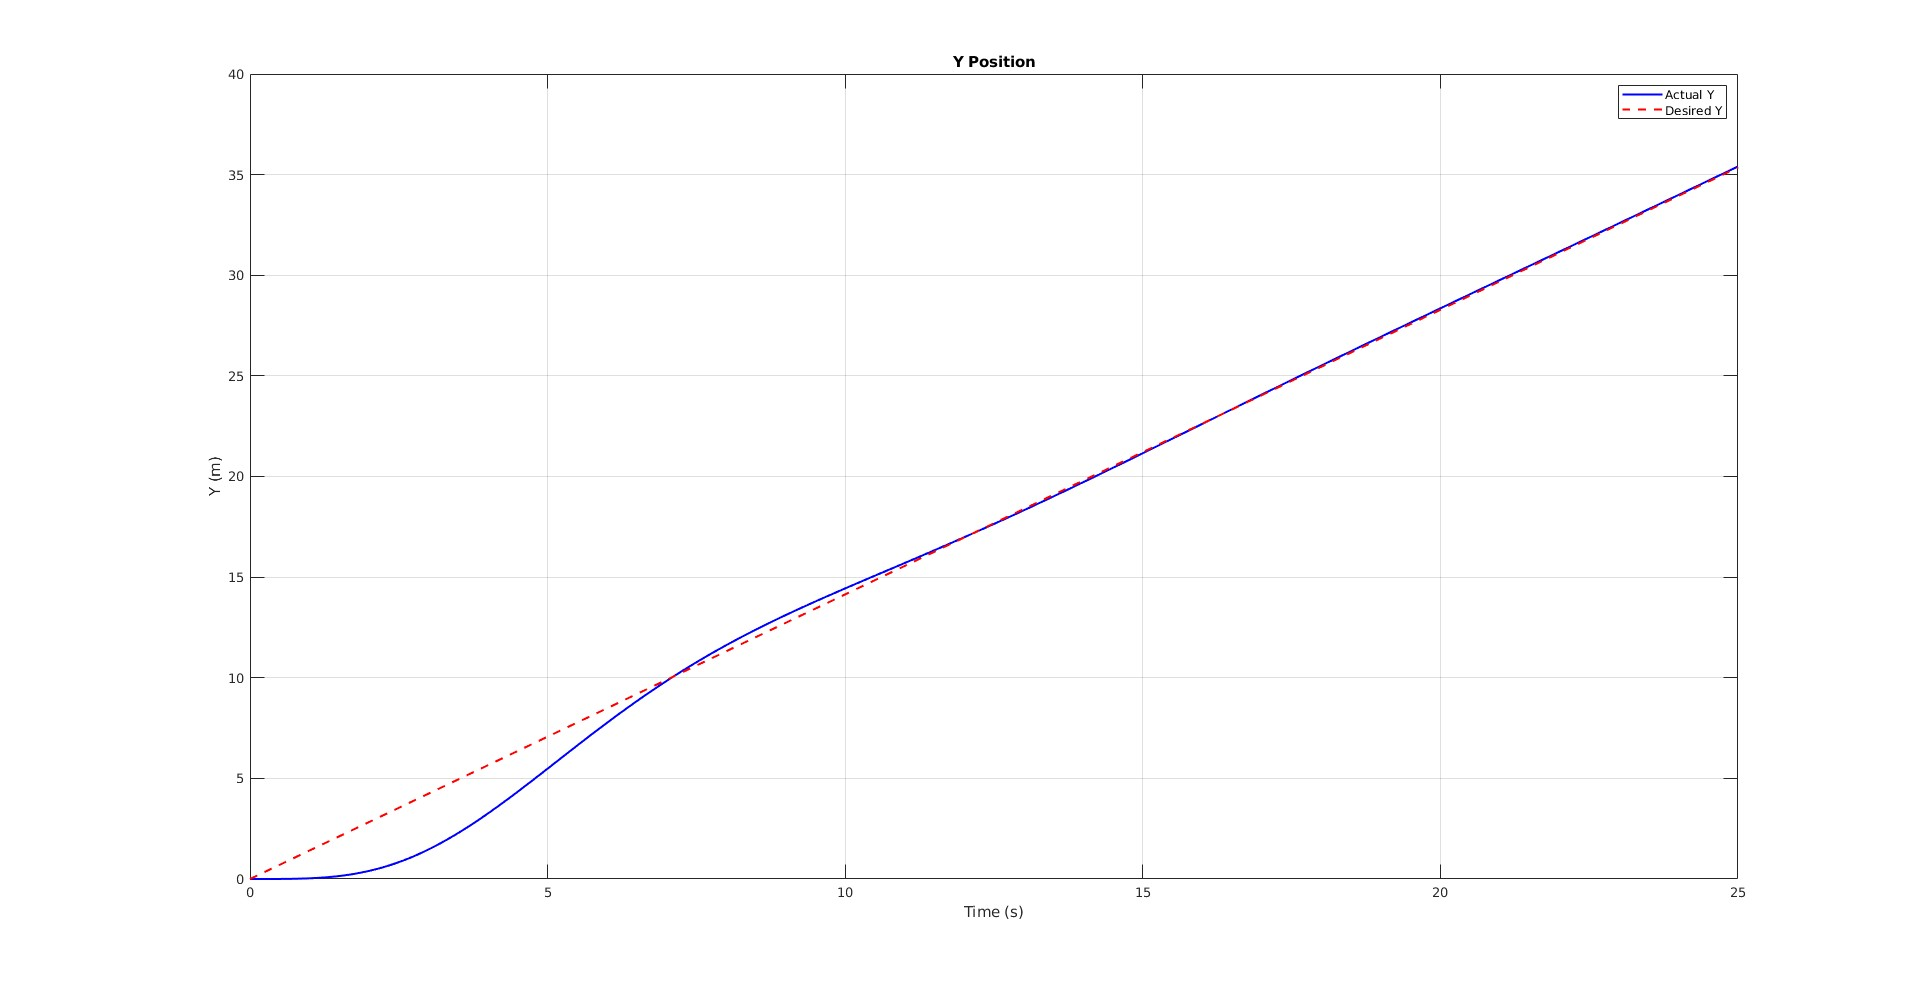
\includegraphics[width=1\textwidth]{images/pd_y.jpg}
    \caption[Caption for Figure 4]{Actual and desired $y$ position}
    \label{fig:pid_y}
\end{figure}
\begin{figure}[h!]
    \centering
     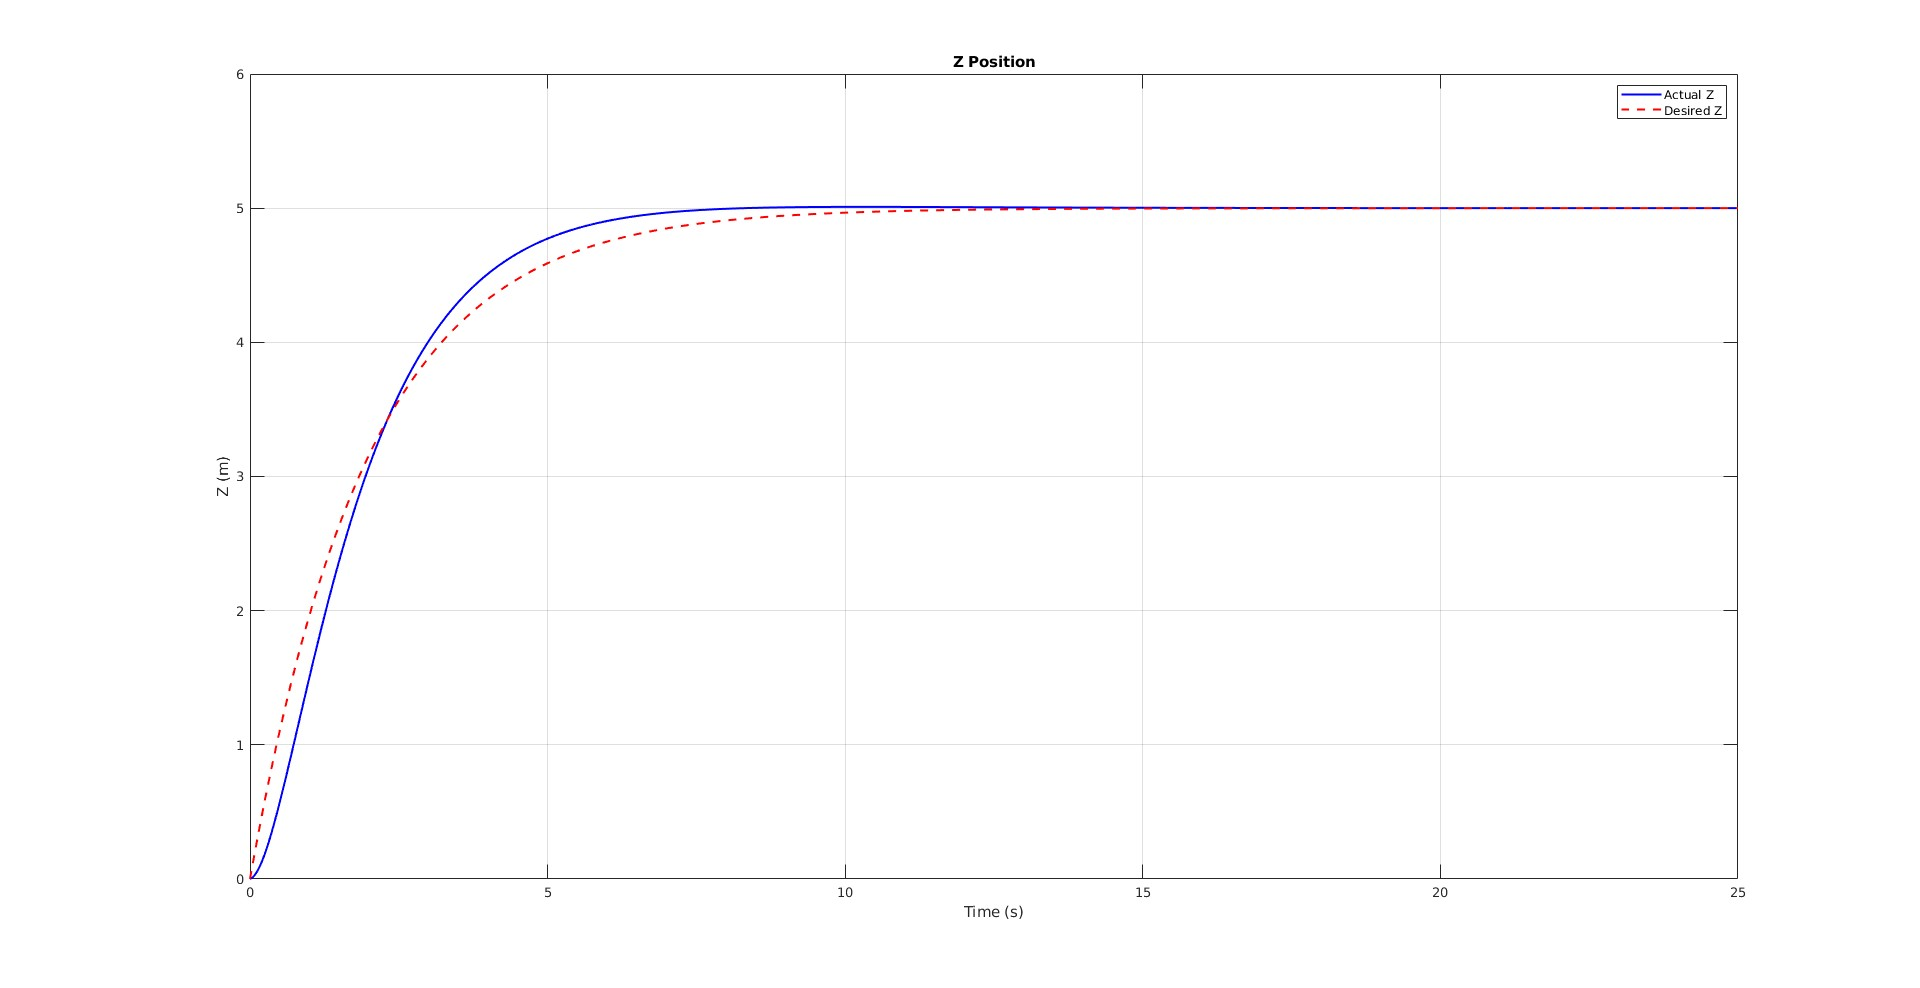
\includegraphics[width=1\textwidth]{images/pd_z.jpg}
    \caption[Caption for Figure 5]{Actual and desired $z$ position}
    \label{fig:pid_z}
\end{figure}

\section{PID Control applied to PSO}
The algorithm integrates the Particle Swarm Optimization (PSO) 
framework with the dynamic motion control of drones to achieve source localization. 
At each iteration of the PSO algorithm, the drones update their velocities and positions 
based on their personal best positions $\mathbf{p}_i^{\text{best}}$, the group best position 
$\mathbf{g}_i^{\text{best}}$, and additional stochastic perturbations. 
The velocity update for each drone is governed by:

\begin{align}
    \mathbf{v}_i^{(t+1)} &= \omega \mathbf{v}_i^{(t)} + c_1 r_1 (\mathbf{p}_i^{\text{best}} - \mathbf{x}_i^{(t)}) + c_2 r_2 (\mathbf{g}_i^{\text{best}} - \mathbf{x}_i^{(t)}),
\end{align}

where $\omega$ is the inertia weight, $c_1$ and $c_2$ are the cognitive and social factors, 
respectively, and $r_1$ and $r_2$ are uniformly distributed random numbers in $[0,1]$. 
Using the updated velocity $\mathbf{v}_i^{(t+1)}$, the new position $\mathbf{x}_i^{(t+1)}$ of each drone is computed as:

\begin{align}
    \mathbf{x}_i^{(t+1)} &= \mathbf{x}_i^{(t)} + \mathbf{v}_i^{(t+1)}.
\end{align}

After computing these updates, the drones execute a one-second movement phase, 
during which they follow the updated velocity vector $\mathbf{v}_i^{(t+1)}$. 
This motion is simulated through a control dynamics model using a time step $\Delta t$. 
The control dynamics ensure realistic drone motion by considering physical constraints such as acceleration and boundary conditions. 
The drone’s state $\mathbf{s}_i$ is updated iteratively:

\begin{align}
    \dot{\mathbf{s}}_i &= f(\mathbf{s}_i, \mathbf{v}_i, \Delta t),
\end{align}

where $f$ models the system dynamics, including position, velocity, and angular rates. 
During this period, the drones operate independently of the PSO loop, allowing them to 
interact with the environment, detect sources, and avoid exclusion zones. This motion phase ensures that
the drones can explore their updated positions in the search space effectively.

At the end of the motion phase, the drones re-enter the PSO loop to evaluate their current positions 
based on the Normalized Source Strength (NSS) function. The best positions are updated if the current 
NSS value exceeds previous records. This iterative alternation between PSO updates and independent drone 
control enables the swarm to balance global exploration and local exploitation, 
ensuring efficient source localization.
